% \textbf{Model uczony na stałej krzywiźnie wierzechołków}

% \begin{figure}[ht]
% 	\centering
% 	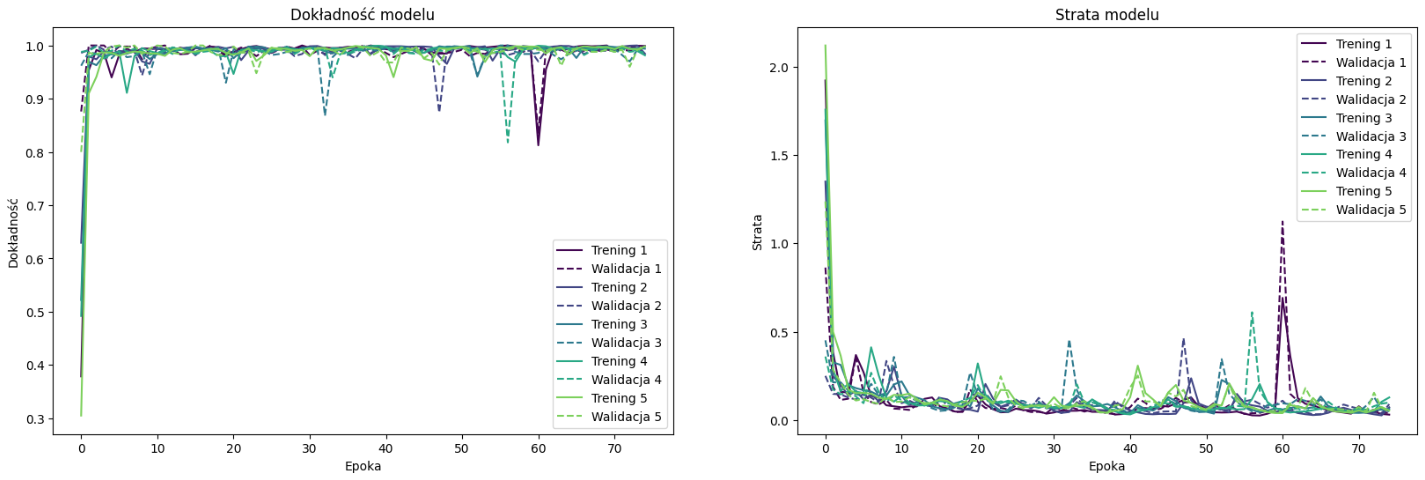
\includegraphics[height=5.5cm]{resources/tests/images/v2/multiple_edges_crossvalid_img.png}
% 	\caption{Wyniki testów dla modelu ze zmienną liczbą wierzchołków i walidacją krzyżową oraz stałą krzywizną wierzchołków}
% 	\label{Fig:tests-csvar-1}
% \end{figure}
% \FloatBarrier

% \begin{figure}[ht]
% 	\centering
% 	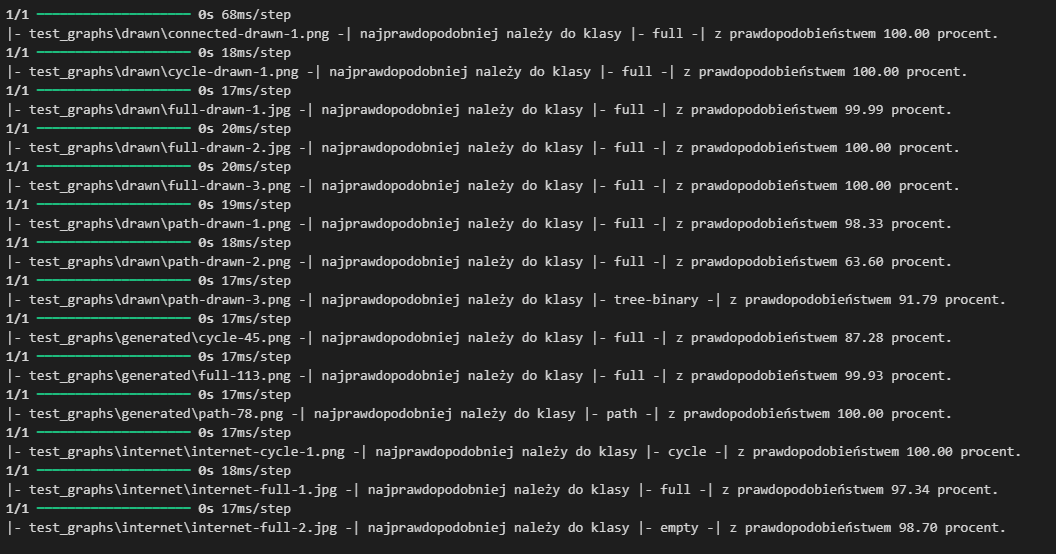
\includegraphics[height=5.5cm]{resources/tests/images/v2/multiple_edges_crossvalid_txt.png}
% 	\caption{Klasyfikacja obrazów zewnętrznych dla modelu ze zmienną liczbą wierzchołków i walidacją krzyżową oraz stałą krzywizną wierzchołków}
% 	\label{Fig:tests-csvar-2}
% \end{figure}
% \FloatBarrier

\textbf{Model uczony na losowej krzywiźnie wierzechołków}

Model uczony na grafach ze zmienną liczbą wierzchołków oraz zastosowaną walidacją krzyżową,
bardzo szybko osiąga poziom dokładności biski 100\%, bo już w kilku pierwszych epokach.
Po około 10 epoce, dokonuje się stabilizacja, oscylująca między 95\%, a 100\%.
W przypadku tego modelu, fluktuacje dokładności są znikome, co wskazuje na dobrą stabilność modelu.
Pojedyncze przypadku spadu dokładności, mogą być spowodowane bardziej skomplikowanymi
przypadkami w zbiorze danych walidacyjnych.

Strata tego modelu gwałtownie spada na początku procesu uczenia,
po czym stabilizuje się na zadowalająco niskim poziomie - poniżej 20\%.
Skoki wskaźnika są bardziej zauważalne na zbiorze walidacyjnym,
ale nie wydają się być regularne i nie wpływają na ogólny wynik.
Mogą być wynikiem, przeuczenia na pojedynczych epokach lub naturalną zmiennością walidacyjnego zbioru danych.

\begin{figure}[ht]
	\centering
	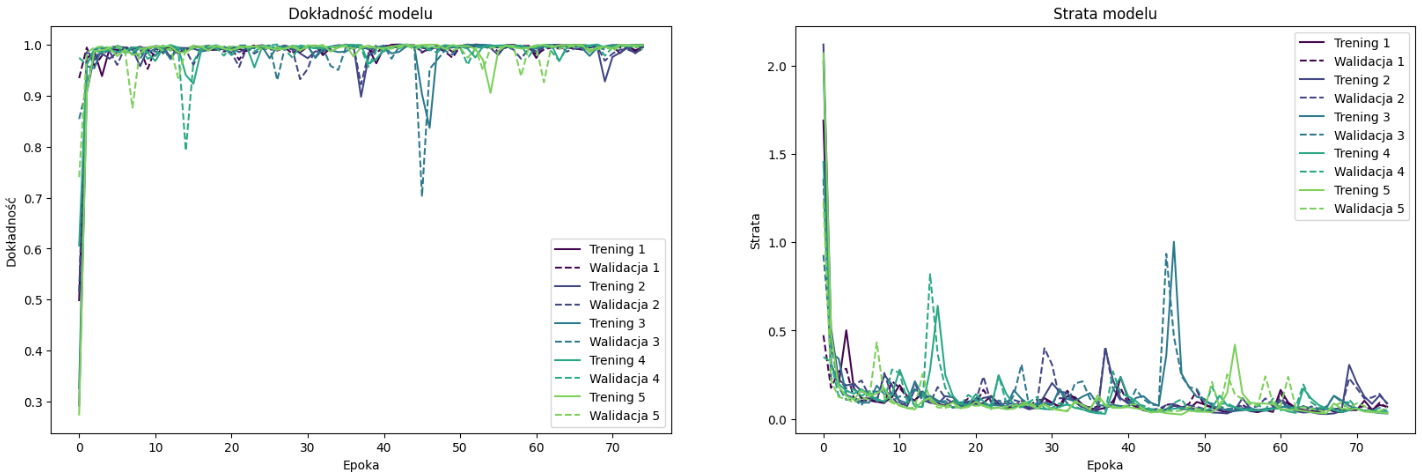
\includegraphics[height=5.5cm]{resources/tests/images/v3/multiple_edges_crossvalid_img.png}
	\caption{Dokładność i walidacja dla modelu ze zmienną liczbą wierzchołków i walidacją krzyżową}
	\label{Fig:tests-csvar-0a}
\end{figure}
\FloatBarrier

Model wydaje się dokładny na zbiorze treningowym i walidacyjnym,
co może skutkować polepszoną skutecznością w klasyfikacji grafów.
Minimalne różnice pomiędzy dokładnością treningową a walidacyjną wskazują na dobrą zdolność generalizacji.
Z otrzymanych wyników, wydawałoby się, że model nie uległ przeuczeniu,
choć jest to również możliwe, zważając na bardzo wysokie wyniki dokładności. 

\begin{figure}[ht]
	\centering
	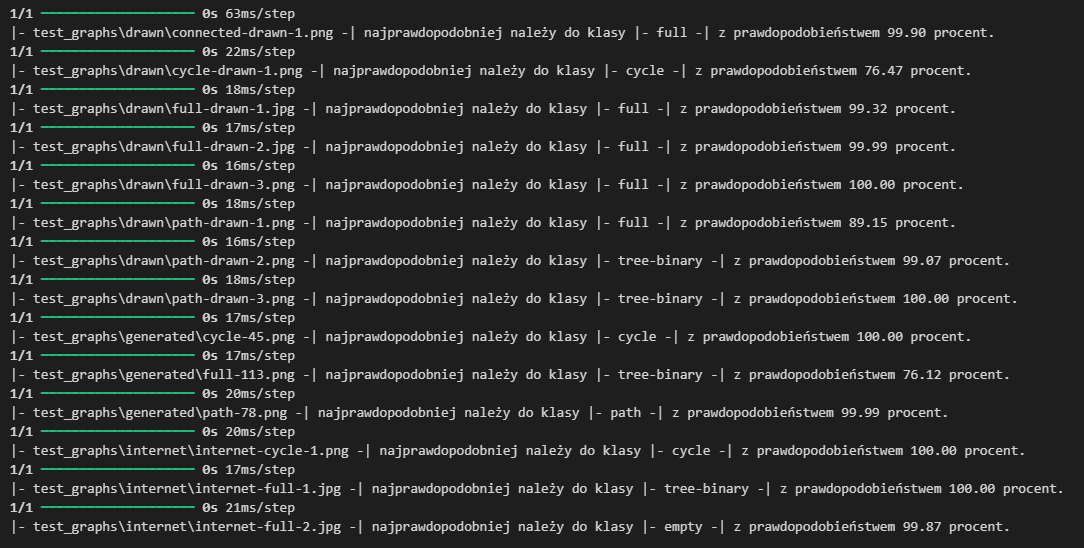
\includegraphics[height=5.5cm]{resources/tests/images/v3/multiple_edges_crossvalid_txt.png}
	\caption{Klasyfikacja obrazów zewnętrznych dla modelu ze zmienną liczbą wierzchołków i walidacją krzyżową}
	\label{Fig:tests-csvar-0b}
\end{figure}
\FloatBarrier

Model poprawnie sklasyfikował połowę testowanych danych zewnętrznych.
Jest to zadowalający wynik, zważając na trudności innych modeli w poprawnym wskazywaniu klas sprawdzanych grafów.

\textbf{Zmodyfikowany model - Conv2D i Droput oraz spowolnienie uczenia}

Opis modyfikacji % ------ TO DO ------ %

Dokładność % ------ TO DO ------ %

Strata % ------ TO DO ------ %

\begin{figure}[ht]
	\centering
	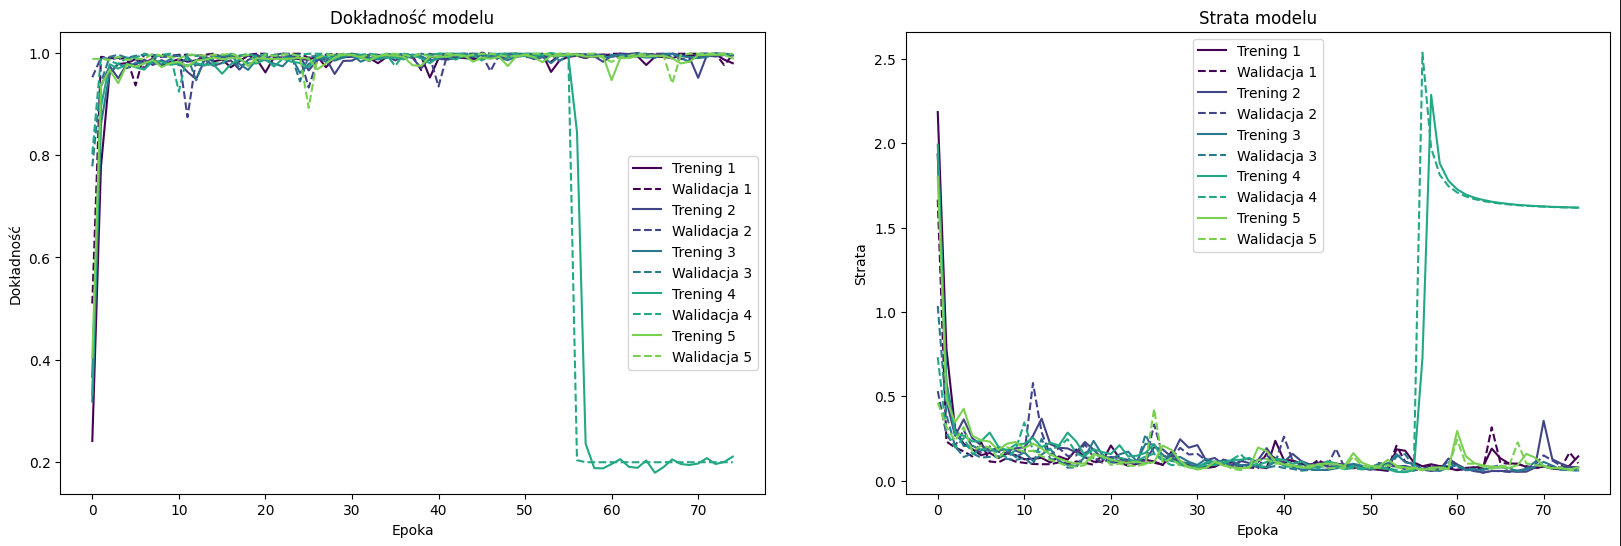
\includegraphics[height=7cm]{resources/tests/images/v4/multiple_edges_crossvalid_1_img.png}
	\caption{Dokładność i walidacja dla zmodyfikowanego modelu ze zmienną liczbą wierzchołków i walidacją krzyżową - Conv2D i Droput}
	\label{Fig:tests-csvar-1a}
\end{figure}
\FloatBarrier

Ogólne % ------ TO DO ------ %

\begin{figure}[ht]
	\centering
	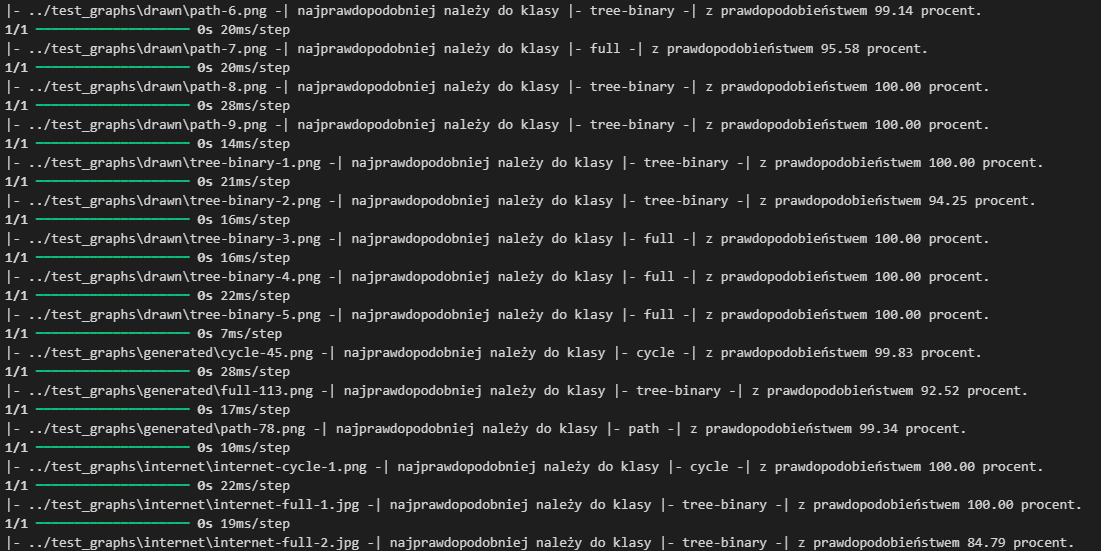
\includegraphics[height=7cm]{resources/tests/images/v4/multiple_edges_crossvalid_1_txt.png}
	\caption{Klasyfikacja obrazów zewnętrznych dla zmodyfikowanego modelu ze zmienną liczbą wierzchołków i walidacją krzyżową - Conv2D i Droput}
	\label{Fig:tests-csvar-1b}
\end{figure}
\FloatBarrier

Opis klasyfikacji % ------ TO DO ------ %

\textbf{Zmodyfikowany model}

Do modelu wprowadzone zostały wszystkie modyfikacje wymienione w rozdziale z modelem z walidacją krzyżową,
czyli zwiększenie liczby filtrów w warstwach, batch normalization, augmentacja danych oraz zmniejszenie szybkości uczenia.

Model dość szybko osiąga wysoką dokładność na zbiorze treningowym - stabilizuje się około 90-95\%.
Podobnie jak i w innych modelach z zastosowanymi wszystkimi modyfikacjami,
dokładność na zbiorze walidacyjnym jest niestabilna.
Można zaobserować duże wahania pomiędzy kolejnymi epokami procesu uczenia.
Sugeruje to trudności z uczeniem się wzorców.

Model szybko zmniejsza stratę treningową i pozostaje ona na bardzo niskim poziomie przez cały proces uczenia.
Wskazuje to na sprawność w uczeniu się na danych treningowych.
Wykresy strat przedstawiają się w nietypowej formie.
Dla początkowych i końcowych epok, straty walidacji niewiele się wahają,
a wręcz przeciwnie sytuacja wygląda dla epok od około dziesiątej do dwudziestej.
Model ma więc trudności z radzeniem sobie z danymi, które są dla niego nowe.

\begin{figure}[ht]
	\centering
	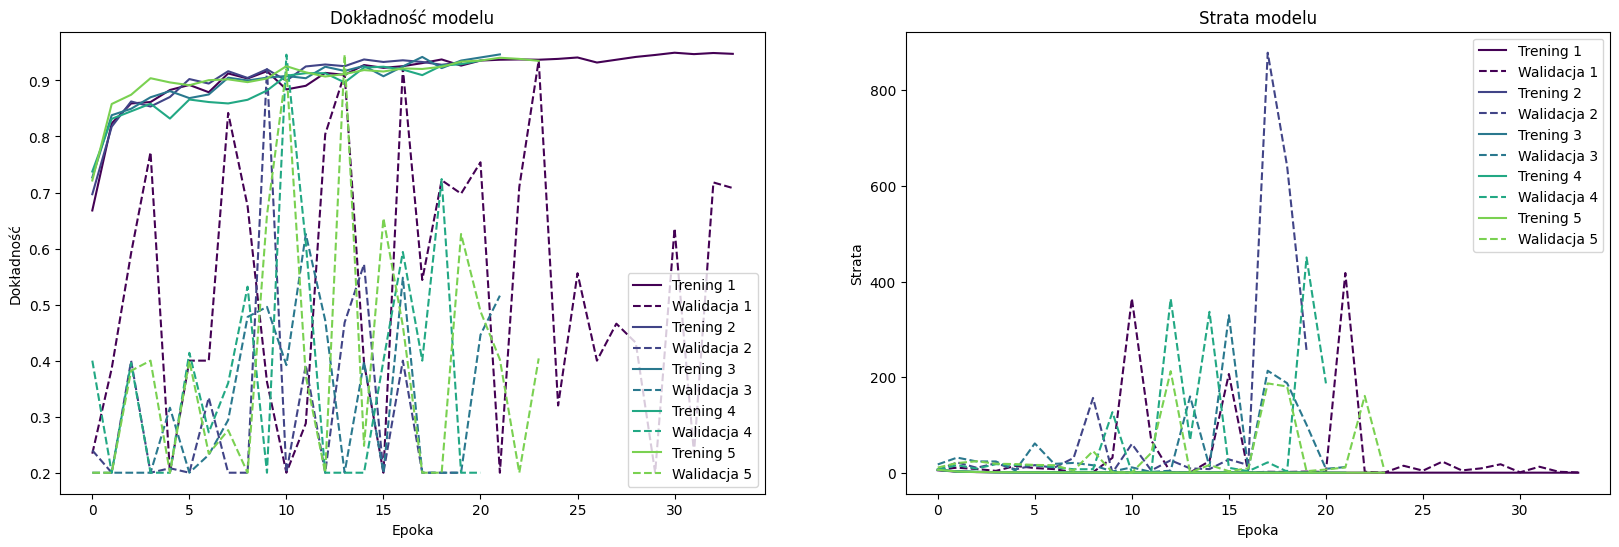
\includegraphics[height=5cm]{resources/tests/images/v4/multiple_edges_crossvalid_img.png}
	\caption{Dokładność i walidacja dla w pełni zmodyfikowanego modelu ze zmienną liczbą wierzchołków i walidacją krzyżową}
	\label{Fig:tests-csvar-2a}
\end{figure}
\FloatBarrier

Model osiąga bardzo wysokie wyniki na zbiorze treningowym,
ale ma problemy z generalizacją na zbiorze walidacyjnym.
Wskazuje to na przeuczenie modelu i brak uczenia się wzorców ogólnych.

\begin{figure}[ht]
	\centering
	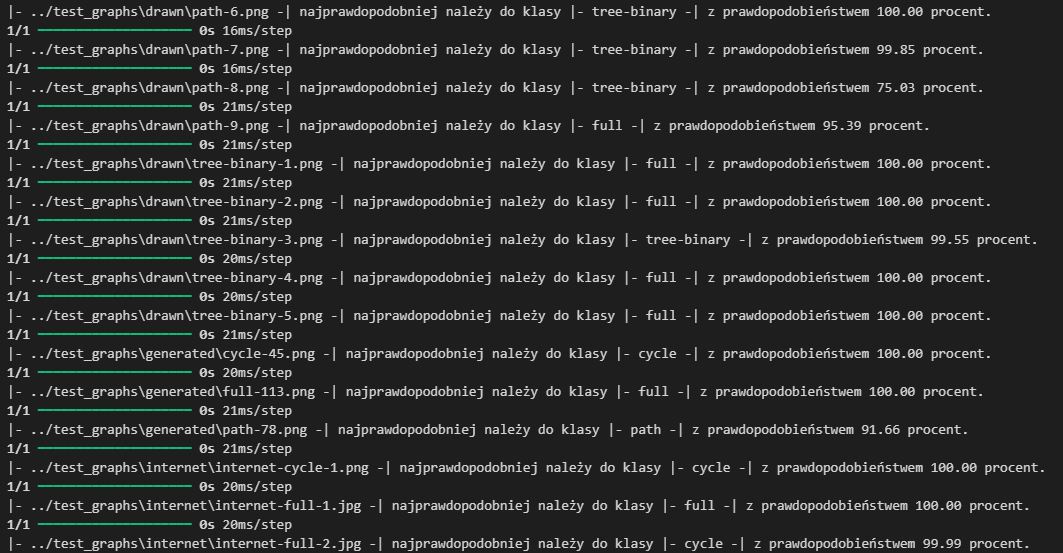
\includegraphics[height=7cm]{resources/tests/images/v4/multiple_edges_crossvalid_txt.png}
	\caption{Klasyfikacja obrazów zewnętrznych dla w pełni zmodyfikowanego modelu ze zmienną liczbą wierzchołków i walidacją krzyżową}
	\label{Fig:tests-csvar-2b}
\end{figure}
\FloatBarrier

Model ocenił poprawnie 6 klas grafów zewnętrznych, z czego większość była grafami wygenerowanymi
(lecz nie stosowanymi w nauce i walidacji), co pokazuje, że model rozpoznaje tylko wzorce,
które są bardzo zbliżone do zbioru treningowego.
Nie jest w stanie rozpoznać poprawnie ani jednego grafu narysowanego ręcznie,
co jest dowodem na to, że nie radzi sobie z nowymi danymi.